\chapter{Control Loop Design and Implementation}
This chapter details the process of combining the project components mentioned in previous chapters.

{\color{red} add more description stuff!}

\section{Description of software implementation}
The main negative consequence of choosing a CNN for object detection is the latency introduced by the long inference time. This influenced the system design to a great extent. In addition, the unexpectedly long time required to get a photo from the Pi camera and preprocess it added to the list of compute-intensive latency-causing components. Thus, it was decided that the system would require the use of multiprocessing and message passing, made possible and simple through the use of python's built in \pyth{multiprocessing} module.

This helped in two ways: the first is that it freed the main process to continuously send commands to the gimbal using the (sometimes predicted) results of the EKF. It would simply not be tolerable to be out of this loop for 200ms or more while a photo is taken and the result inferred.

The second advantage is that while implementing a parallel data pipeline would increase the overall latency between a photo being taken and the result being used, the final number of readings per second actually increases. This is because while one process takes a photo, another can simultaneously infer the image while the parent process communicates with the gimbal controller.

Thus, data was passed from one process to the next using parallel processing Queues. A block diagram of this and the other components in the pipeline is shown in Figure~\ref{fig:system_block_diagram}.

\begin{figure}[h!]
  \centering
  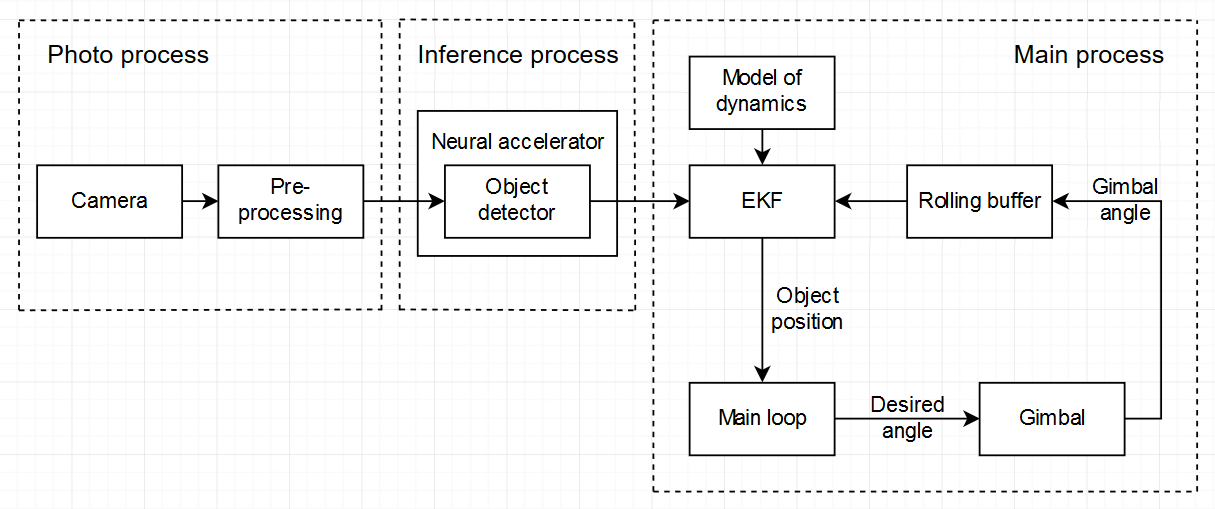
\includegraphics[width=\textwidth]{methodology/system_block_diagram2}
  \caption{\label{fig:system_block_diagram} FILL ME IN.}
\end{figure}

A more detailed description of the rest of the general flow diagram and the reasoning behind the choices made is detailed in the following subsections.

\subsection{The photo process}
In the photo stage, a child process would interface with the Raspberry Pi camera. It received all photos taken, do some preprocessing on each image, and then passed the resulting array to the next stage in the pipeline. It also sent the time at which the photo was taken. A single loop in this stage took around 60-150ms, depending on the chosen camera resolution.

\subsection{The inference process}
In the inference stage, another child process interfaced with the Movidius NCS. It received the preprocessed images from the previous stage and loaded them onto the neural accelerator. While waiting for the inference result, it would occasionally save a copy of the photo to disk for offline debugging purposes. Once it received the result, it would decode the neural net output, put it and the photo time into an easy to use python dictionary and place it in a final buffer. Again, this needed to be in a separate process as the total time required to pass an image to the NCS and then infer a result was about 100ms.

\subsection{The main process}
While this was happening, the main parent process continuously runs a control loop which receives the results from the inference process, and uses it to update two EKFs which track the object's pitch and yaw states. It also communicates with the gimbal controller using its serial API. Lastly, it logs relevant data for debugging purposes.



\section{Fixing timing issues}
The large latency in the object detection caused further problems which needed to be fixed. These problems and their solutions are described in the following subsections.

\subsection{EKF timing issues}
Recall that the neural network can only give a relative angle between the camera and the object, while the gimbal works using absolute angles with respect to some initial position.

The EKFs, each tracking the absolute angular states of the object, would need to be passed the results from the neural network as absolute angles. This could be done by reading requesting the gimbal to send its angular position at the time that the photo was taken. \\

\begin{python}
gc_angles = gc.get_motor_angles()
EKF_yaw.update(phi_yaw + gc_angles['yaw'])
EKF_pitch.update(phi_pitch + gc_angles['pitch'])
\end{python}

However, this presented a new problem to be solved - the angular state of the camera at the time that the photo was taken usually significantly different by the time the result had been inferred due to the large latency in the inference.

\begin{enumerate}
\item $t = 0$: photo taken and inference started.
\item $t = 200ms$: result received for for $t=0$. By this time, the gimbal has moved slightly, causing a mismatch between the relative angles from the recent inference and the current absolute gimbal angles.
\end{enumerate}

The solution was to keep a rolling buffer of a few gimbal angle readings, and then use the angle measurement at the time closest to the photo time to properly convert the neural network measurement from a relative angle to a global one. The snippets of code relevant to this are shown below. \\

\begin{python}
# current time, put into rolling buffer
gc_logger_time[gc_i % gc_logger_len] = time.time()

# gimbal angle at current time
gc_logger_yaw[gc_i % gc_logger_len] = gc_angles['yaw']
gc_i += 1

# later on...
# index of the logger time closest to the photo time
idx = np.argmin(np.abs(gc_logger_time - photo_time))
EKF_yaw.update(phi_yaw + gc_logger_yaw[idx])
\end{python}

Another reason why this approach was necessary was because the time between taking a photo and getting the result was non-constant.

\subsection{Control timing issues}
Given that the EKF in the gimbal was working correctly, there were two options for how to handle the latency of the pipeline.

\begin{enumerate}
\item $t = 0$: photo taken and inference started.
\item $t = 200ms$: result received for for $t=0$. By this time, the object has moved slightly.
\item Two options:
	\begin{itemize}
	\item Use estimate from $t=0$
	\item Use EKF to predict from $t=0$ to $t=200ms$
	\end{itemize}
\end{enumerate}

The first approach was to track the EKFs estimate of the object at all times. Since the EKFs receive all data with a roughly $\approx 200ms$ delay, the resulting system would essentially track the position of tracked object $200ms$ after in the past. This approach accepts the fact that the camera will usually not aim at the camera but instead lag a few degrees behind it (depending on the angular velocity of the object).

The second approach would be to use the EKF estimate of the angular state of the object to 'predict' from the EKF's $\approx 200ms$ lagging time into the actual live time. If successful, the camera would perfectly track the position of the object as it moves along. However, there is no guarantee that the EKF prediction will match the actual movements of the object. Thus, this approach would be prone to things like extreme overshoot every time the object slowed down or turned around.

There is merit to both approaches - the first is more robust, with worse camera tracking. The second is less robust, but would result if better footage if the object moved at a relatively constant velocity. Thus, the choice depends largely on application. For the purposes of this project, robustness was valued more highly. This meant going with the first approach of tracking the object a fifth of a second in the past.


\section{Benchmarking the flow of data}
{\Large \color{red} (maybe rather put this in the results section?)}

{\Large \color{red} talk about the time it takes to: take a picture, pre-process the image, load it onto the NCS, get the inference result}

{\Large \color{red} the effect of python's garbage collection}

